\section{Labview Tutorial }
\subsection{Transmitter Overview}

    Following figure is the transmitter Labview diagram. \\
    
    \vspace{-4mm}  
    \begin{figure}[!h]\raggedleft
    \hspace{15mm}
		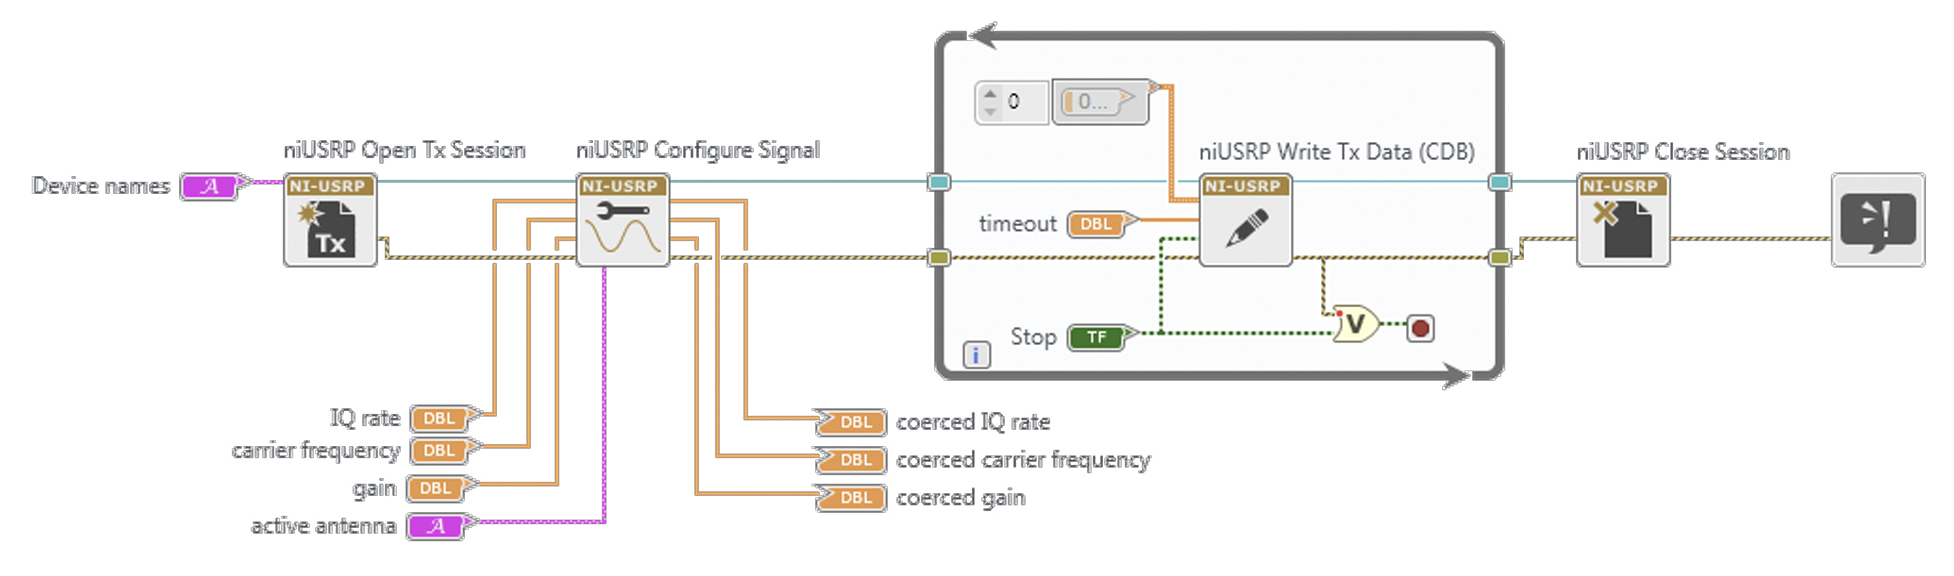
\includegraphics[width=.95\textwidth]{image/week03/2-1-1.png}
		\caption{\footnotesize Transmitter Labview diagram}
		\vspace{-10pt}
    \end{figure}
    
    There are 4 main blocks regarding USRP transmitter \\
    1. Open TX session : Turn on USRP and link the code to it. \\
    2. Configure Signal : Configure signal parameters for USRP antenna (IQ rate, carrier frequency, gain, etc.) \\
    3. Write TX data : Transmit data via USRP antenna \\
    4. Close Session : Turn off USRP \\
\clearpage

    %%%%%%%%%%%%%%%%%%%%%%%%%%%%%%%%%%%%%%%%%%%%%%%%%
    
\subsection{Basic Tutorial with Example Labview Code}
    
    \subsubsection*{Parameters}
    \begin{table}[!h]\centering
        \hspace{10mm}
        \begin{tabular}{|l|c|c|}
        \hline
        \multicolumn{1}{|l|}{Parameter} & \multicolumn{1}{l|}{Value} \\
        \hline
        Number of Chirps & 4 \\ 
        \hline
        Chirp Direction & Up \\ 
        \hline
        Carrier Frequency & 2.4G \\ 
        \hline
        IQ rate & 4M \\ 
        \hline
        \end{tabular}
        \caption{Experiment 2 parameter values}
    \end{table}
    
    \subsubsection*{Experiment Result}
    \vspace{-4mm}  
    \begin{figure}[!h]\raggedleft
    \hspace{15mm}
		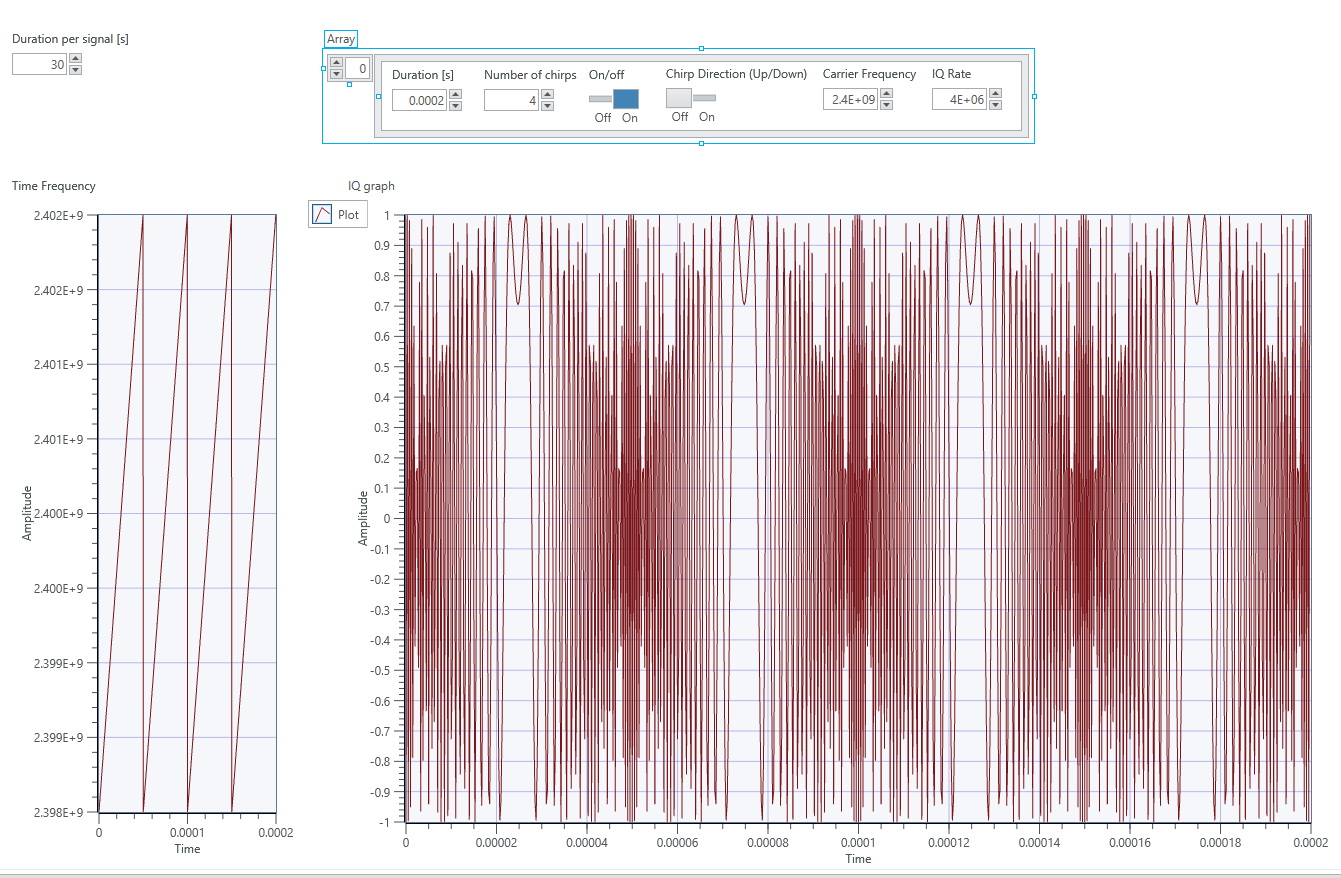
\includegraphics[width=.95\textwidth]{image/week03/2-2-1.png}
		\caption{\footnotesize Experiment 2 result}
		\vspace{-10pt}
    \end{figure}
\clearpage